\chapter{Computability}\label{ch:computability}\label{ch:universal}
\begin{schemeregion}

\chapquotew{However unapproachable these problems may seem to us and however helpless we stand before them, we have, nevertheless, the firm conviction that their solution must follow by a finite number of purely logical processes$\ldots$This conviction of the solvability of every mathematical problem is a powerful incentive to the worker.  We hear within us the perpetual call: There is the problem.  Seek its solution.  You can find it by pure reason; for in mathematics there is no ignorabimus.}{David~Hilbert, 1900}{10.5cm}\index{people}{Hilbert, David}
%\emph{Address~to~the~Second~International~Congress~of~Mathematicians}, 1900}

%\chapquoter{\Godel's paper has reached me at last.  I am very suspicious of it now but will have to swot up the Zermelo-van Neumann system a bit before I can put objections down in black \& white.}{Alan Turing, letter to Max Newman, 1940}\index{Turing, Alan}\index{\Godel, Kurt}

In this chapter we consider the question of what problems can and cannot be solved by mechanical computation.  This is the question of \definition{computability}: a problem is \emph{computable} if it can be solved by some algorithm; a problem that is \emph{noncomputable} cannot be solved by any algorithm.\index{general}{computable}\index{general}{noncomputable}

Section~\ref{sec:mechanized-reasoning} considers first the analogous question for declarative knowledge: are there true statements that cannot be proven by \emph{any} proof? Section~\ref{sec:haltingproblem} introduces the \emph{Halting Problem}, a problem that cannot be solved by any algorithm.  Section~\ref{sec:universality} sketches Alan Turing's proof that the Halting Problem is noncomputable.  Section~\ref{sec:noncomputability} discusses how to show other problems are noncomputable.

\section{Mechanizing Reasoning}\label{sec:mechanized-reasoning}

Humans have been attempting to mechanize reasoning for thousands of years.  Aristotle's \emph{Organon} developed rules of inference known as \definition{syllogisms} to codify logical deductions in approximately 350 BC. \index{people}{Aristotle}\index{general}{Organon} 
\cut{For example:
\begin{quote}
\begin{center}
Every \emph{A} is a \emph{P}.\\
\underline{\qquad\emph{X} is an \emph{A}.\qquad}\\
\emph{X} is a \emph{P}.\\
\end{center}
\end{quote}
The statements above the line are the premises, and the statement under the line is the conclusion. The variables $A$, $P$, and $X$ can be bound to any value.  If the first two statements are true, then the inference rule states that the third statement must also be true.  For example, binding $A$ to \sresult{human}, $P$ to \sresult{mortal}, and $X$ to \sresult{\Godel}, we get:
\begin{quote}
\begin{center}
Every human is mortal.\\
\underline{\qquad\Godel\ is a human.\qquad}\\
\Godel\ is mortal.\\
\end{center}
\end{quote}
}

Euclid went beyond Aristotle by developing a formal axiomatic system.  An \definition{axiomatic system} is a formal system consisting of a set of \emph{axioms} and a set of \emph{inference rules}.  The goal of an axiomatic system is to codify knowledge in some domain.  \index{people}{Euclid}\index{general}{Elements}

The axiomatic system Euclid developed in \emph{The Elements} concerned constructions that could be drawn using just a straightedge and a compass.  \cut{Euclid collected many theorems that had been previously proved by others including Eudoxus, Pythagoras, and Theaetetus, but presented them in a more rigorous way.  Euclid's \emph{Elements} is the most successful textbook of all time, something every educated person was expected to read until recently.}

Euclid started with five axioms (more commonly known as \emph{postulates}); an example axiom is: \emph{A straight line segment can be drawn joining any two points.}  \index{general}{postulate}\cut{
:\footnote{Euclid's original writings, of course, were in Greek.  This version of the postulates is adapted from Eric Weisstein, \emph{Euclid's Postulates} (From \emph{MathWorld---A Wolfram Web Resource}, \url{http://mathworld.wolfram.com/EuclidsPostulates.html}); many other translations exist, but the essential meaning of the postulates is the same.}
 
\begin{enumerate}
\item A straight line segment can be drawn joining any two points.
\item Any straight line segment can be extended indefinitely in a straight line.
\item Given any straight line segment, a circle can be drawn having the segment as radius and one endpoint as center.
\item All right angles are equal.
\item If two lines are drawn which intersect a third in such a way that the sum of the inner angles on one side is less than two right angles, then the two lines must intersect each other on that side if they are extended far enough.
\end{enumerate}

} In addition to the postulates, Euclid states five \emph{common notions}, which could be considered inference rules.  An example of a common notion is: \emph{The whole is greater than the part.}
\cut{
Euclid also stated 23 definitions, assigning names to things.  An example of a definition is:
\begin{quote}
A \emph{circle} is a plane figure contained by one line such that all the straight lines falling upon it from one point among those lying within the figure equal one another.
\end{quote}
}

Starting from the axioms and common notions, along with a set of definitions (e.g., defining a \emph{circle}), Euclid proved 468 propositions mostly about geometry and number theory.  A \definition{proposition} is a statement that is stated precisely enough to be either true or false.  Euclid's first proposition is: given any line, an equilateral triangle can be constructed whose edges are the length of that line.

A \definition{proof} of a proposition in an axiomatic system is a sequence of steps that ends with the proposition.  Each step must follow from the axioms using the inference rules.  Most of Euclid's proofs are constructive: propositions state that a thing with a particular property exists, and proofs show steps for constructing something with the stated property.  The steps start from the postulates and follow the inference rules to prove that the constructed thing resulting at the end satisfies the requirements of the proposition.

\LATER{
For example, here is Euclid's proof of the first proposition:
}

A \definition{consistent} axiomatic system is one that can never derive contradictory statements by starting from the axioms and following the inference rules. If a system can generate both $A$ and \emph{not} $A$ for any proposition $A$, the system is inconsistent.  If the system cannot generate any contradictory pairs of statements it is consistent.  %Euclid's system is consistent; there is no way to derive contradictory statements in the system.

A \definition{complete} axiomatic system can derive all true statements by starting from the axioms and following the inference rules.  This means if a given proposition is true, some proof for that proposition can be found in the system.  Since we do not have a clear definition of \emph{true} (if we defined true as something that can be derived in the system, all axiomatic systems would automatically be complete by definition), we state this more clearly by saying that the system can decide any proposition.  This means, for any proposition \emph{P}, a complete axiomatic system would be able to derive either \emph{P} or \emph{not P}.  A system that cannot decide all statements in the system is \emph{incomplete}.  	An ideal axiomatic system would be complete and consistent: it would derive all true statements and no false statements.  

The completeness of a system depends on the set of possible propositions.  Euclid's system is consistent but not complete for the set of propositions about geometry.  There are statements that concern simple properties in geometry (a famous example is \emph{any angle can be divided into three equal sub-angles}) that cannot be derived in the system; trisecting an angle requires more powerful tools than the straightedge and compass provided by Euclid's postulates.

Figure~\ref{fig:axiomatic-systems} depicts two axiomatic systems.  The one on the left one \emph{incomplete}: there are some propositions that can be stated in the system that are true for which no valid proof exists in the system.  The one on the right is \emph{inconsistent}: it is possible to construct valid proofs of both \emph{P} and \emph{not P} starting from the axioms and following the inference rules.  Once a single contradictory proposition can be proven the system becomes completely useless.  The contradictory propositions amount to a proof that \scheme|true = false|, so once a single pair of contradictory propositions can be proven every other false proposition can also be proven in the system.  Hence, only consistent systems are interesting and we focus on whether it is possible for them to also be complete.

\begin{figure}[!bth]
\begin{center}
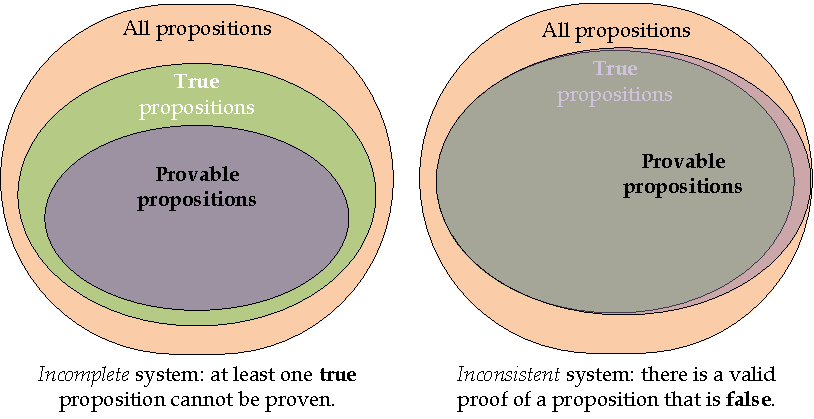
\includegraphics[width=4.8in]{figures/axiomaticsystems.pdf}
\caption{Incomplete and inconsistent axiomatic systems.}\label{fig:axiomatic-systems}
\end{center}
\end{figure}

\shortsection{Russell's Paradox} Towards the end of the 19$^{th}$ century, many mathematicians sought to systematize mathematics by developing a consistent axiomatic system that is complete for some area of mathematics.  One notable attempt was Gottlob Frege's \emph{Grundgestze der Arithmetik} (1893) which attempted to develop an axiomatic system for all of mathematics built from simple logic.

Bertrand Russell discovered a problem with Frege's system, which is now known as \definition{Russell's paradox}.  Suppose $R$ is defined as the set containing all sets that do not contain themselves as members.  For example, the set of all prime numbers does not contain itself as a member, so it is a member of $R$.  On the other hand, the set of all entities that are not prime numbers is a member of $R$.  This set contains all sets, since a set is not a prime number, so it must contain itself.  \index{people}{Russell, Bertrand}

The paradoxical question is: \emph{is the set $R$ a member of $R$?}  There are two possible answers to consider but neither makes sense:
\begin{descriptionlist}
\item[Yes: $R$ is a member of $R$]\forcenl
We defined the set $R$ as the set of all sets that do not contain themselves as member.  Hence, $R$ cannot be a member of itself, and the statement that $R$ is a member of $R$ must be false.
\item[No: $R$ is not a member of $R$]\forcenl
If $R$ is not a member of $R$, then $R$ does not contain itself and, by definition, must be a member of set $R$.  This is a contradiction, so the statement that $R$ is not a member of $R$ must be false.
\end{descriptionlist}
%This is a paradox!  
The question is a perfectly clear and precise binary question, but neither the ``yes'' nor the ``no'' answer makes any sense.  Symbolically, we summarize the paradox: for any set $s$, $s \in R$ if and only if $s \notin s$.  Selecting $s = R$ leads to the contradiction: $R \in R$ if and only if $R \notin R$.

Whitehead and Russell attempted to resolve this paradox by constructing their system to make it impossible to define the set $R$.  Their solution was to introduce types.  Each set has an associated type, and a set cannot contain members of its own type.  The set types are defined recursively:
\begin{itemtight}
\item A \emph{type zero set} is a set that contains only non-set objects.  
\item A \emph{type-$n$ set} can only contain sets of type $n-1$ and below.  
\end{itemtight}
This definition avoids the paradox: the definition of $R$ must now define $R$ as a set of type $k$ set containing all sets of type $k-1$ and below that do not contain themselves as members.  Since $R$ is a type $k$ set, it cannot contain itself, since it cannot contain any type $k$ sets.  

In 1913, Whitehead and Russell published \definition{Principia Mathematica}, a bold attempt to mechanize mathematical reasoning that stretched to over 2000 pages.  Whitehead and Russell attempted to derive all true mathematical statements about numbers and sets starting from a set of axioms and formal inference rules.  They employed the type restriction to eliminate the particular paradox caused by set inclusion, but it does not eliminate all self-referential paradoxes.  

For example, consider this paradox named for the Cretan philosopher Epimenides who was purported to have said ``All Cretans are liars''.  If the statement is true, than Epimenides, a Cretan, is not a liar and the statement that all Cretans are liars is false.  Another version is the self-referential sentence: \emph{this statement is false}.  If the statement is true, then it is true that the statement is false (a contradiction).  If the statement is false, then it is a true statement (also a contradiction).  It was not clear until \Godel, however, if such statements could be stated in the \emph{Principia Mathematica} system.\index{general}{Epimenides paradox}  

\subsection{\Godel's Incompleteness Theorem}\index{people}{G\"{o}del, Kurt}\index{general}{incompleteness}

Kurt \Godel\ was born in Brno (then in Austria-Hungary, now in the Czech Republic) in 1906. \Godel\ proved that the axiomatic system in \emph{Principia Mathematica} could not be complete and consistent.  More generally, \Godel\ showed that \emph{no} powerful axiomatic system could be both complete and consistent: no matter what the axiomatic system is, if it is powerful enough to express a notion of proof, it must also be the case that there exist statements that can be expressed in the system but cannot be proven either true or false within the system.  
\sidepicture{0.22}{images/Godel_Einstein_1950.jpg}{\Godel\ with Einstein, 1950}{Princeton, Institute for Advanced Study Archives} 
%http://en.wikipedia.org/wiki/File:Godel_Einstein_1950.jpeg

\Godel's proof used construction: to prove that \emph{Principia Mathematica} contains statements which cannot be proven either true or false, it is enough to find one such statement. The statement \Godel\ found:
\begin{smallquote}
\begin{tabular}{p{2em}p{24em}}
$G_{PM}$: & {\raggedright Statement $G_{PM}$ does not have any proof in the system of \emph{Principia Mathematica}.} \tabularnewline
\end{tabular}
\end{smallquote}

Similarly to Russel's Paradox, this statement leads to a contradiction.  It makes no sense for $G_{PM}$ to be either true or false:
\begin{descriptionlist}
\item[Statement $G_{PM}$ is provable in the system.]\forcenl
If $G_{PM}$ is proven, then it means $G_{PM}$ does have a proof, but $G_{PM}$ stated that $G_{PM}$ has no proof.  The system is inconsistent: it can be used to prove a statement that is not true.  
\item[Statement $G_{PM}$ is not provable in the system.]\forcenl
Since $G_{PM}$ cannot be proven in the system, $G_{PM}$ is a true statement.  The system is incomplete: we have a true statement that is not provable in the system.
\end{descriptionlist}

The proof generalizes to \emph{any} axiomatic system, powerful enough to express a corresponding statement \emph{G}:
\begin{smallquote}
$G$: Statement $G$ does not have any proof in the system.
\end{smallquote}
For the proof to be valid, it is necessary to show that statement \emph{G} can be expressed in the system.  

To express $G$ formally, we need to consider what it means for a statement to not have any proof in the system.  A proof of the statement $G$ is a sequence of steps, $T_0$, $T_1$, $T_2$, $\ldots$, $T_N$. Each step is the set of all statements that have been proven true so far.  Initially, $T_0$ is the set of axioms in the system.  To be a proof of $G$, $T_N$ must contain $G$.  To be a valid proof, each step should be producible from the previous step by applying one of the inference rules to statements from the previous step.  

To express statement $G$ an axiomatic system needs to be powerful enough to express the notion that a valid proof does not exist.  \Godel\ showed that such a statement could be constructed using the \emph{Principia Mathematica} system, and using any system powerful enough to be able to express interesting properties.  That is, in order for an axiomatic system to be complete and consistent, it must be so weak that it is not possible to express \emph{this statement has no proof} in the system.

\section{The Halting Problem}\label{sec:haltingproblem}\index{general}{halting problem}

\Godel\ established that no interesting and consistent axiomatic system is capable of proving all true statements in the system.  Now we consider the analogous question for computing: \emph{are there problems for which no algorithm exists?}  

Recall these definitions form Chapters~\ref{ch:intro} and ~\ref{ch:problems}:
\begin{descriptionlist}
\item [\emph{problem}:] A description of an input and a desired output.  
\item [\emph{procedure}:] A specification of a series of actions.  
\item [\emph{algorithm}:] A procedure that is guaranteed to always terminate.   
\end{descriptionlist}
A procedure solves a problem if that procedure produces a correct output for every possible input.  If that procedure always terminates, it is an algorithm.  So, the question can be stated as: \emph{are there problems for which no procedure exists that produces the correct output for every possible problem instance in a finite amount of time?}   

A problem is \definition{computable} if there exists an algorithm that solves the problem. It is important to remember that in order for an algorithm to be a solution for a problem $P$, it must always terminate (otherwise it is not an algorithm) and must always produce the correct output for \emph{all} possible inputs to $P$. If no such algorithm exists, the problem is \definition{noncomputable}.\footnote{The terms \emph{decidable} and \emph{undecidable} are sometimes used to mean the same things as computable and noncomputable.}

\LATER{
\subsection{Hilbert and the Entscheidungsproblem}

\TODO{Add Hilbert history}
}

Alan Turing proved that noncomputable problems exist.  The way to show that uncomputable problems exist is to find one, similarly to the way \Godel\ showed unprovable true statements exist by finding an unprovable true statement.  

The problem Turing found is known as the \emph{Halting Problem}:\footnote{This problem is a variation on Turing's original problem, which assumed a procedure that takes one input. Of course, Turing did not define the problem using a Python program since Python had not yet been invented when Turing proved the Halting Problem was noncomputable in 1936.  In fact, nothing resembling a programmable digital computer would emerge until several years later.}

\problem{Halting Problem}{A string representing a Python program.}{If evaluating the input program would ever finish, output \True.  Otherwise, output \False.}

Suppose we had a procedure \pycode|halts| that solves the Halting Problem.  The input to \pycode|halts| is a Python program expressed as a string.  
%We could not use the Scheme expression directly as the input, since that would mean that it is evaluated before \scheme|halts?| is applied; if this were done, the \scheme|halts?| procedure would never %be applied if the input expression would not halt.

For example, \pycode|halts('(+ 2 3)')| should evaluate to \True, \pycode|halts('while True: pass')| should evaluate to \False\ (the Python \pycode|pass| statement does nothing, but is needed to make the while loop syntactically correct), and
\begin{pythoncode}
halts(''''''
        def fibo(n):
           if n == 1 or n == 2: return 1
           else: return fibo(n-1) + fibo(n-2)
        fibo(60)
    '''''')
\end{pythoncode}
should evaluate to \True.  From the last example, it is clear that \pycode|halts| cannot be implemented by evaluating the expression and outputting \True\ if it terminates.  The problem is knowing when to give up and output \False.  As we analyzed in Chapter~\ref{ch:cost}, evaluating \pycode|fibo(60)| would take trillions of years; in theory, though, it eventually finishes so \pycode|halts| should output \True.

This argument is not sufficient to prove that \pycode|halts| is noncomputable.  It just shows that one particular way of implementing \pycode|halts| would not work.  To show that \pycode|halts| is noncomputable, we need to show that it is impossible to implement a \pycode|halts| procedure that would produce the correct output for all inputs in a finite amount of time.

Here is another example that suggests (but does not prove) the impossibility of \pycode|halts| (where \pycode|sumOfTwoPrimes| is defined as an algorithm that take a number as input and outputs \True\ if the number is the sum of two prime numbers and \False\ otherwise):
\begin{pythoncode} 
halts('n = 4; while sumOfTwoPrimes(n): n = n + 2')
\end{pythoncode}
This program halts if there exists an even number greater than 2 that is not the sum of two primes.  We assume unbounded integers even though every actual computer has a limit on the largest number it can represent.  Our computing model, though, uses an infinite tape, so there is no arbitrary limit on number sizes.  

Knowing whether or not the program halts would settle an open problem known as Goldbach's Conjecture: {\em every even integer greater than 2 can be written as the sum of two primes.}  Christian Goldbach proposed a form of the conjecture in a letter to Leonhard Euler in 1742.  Euler refined it and believed it to be true, but couldn't prove it.

With a \pycode|halts| algorithm, we could settle the conjecture using the expression above: if the result is \False, the conjecture is proven; if the result is \True, the conjecture is disproved.  We could use a \pycode|halts| algorithm like this to resolve many other open problems.\index{people}{Euler, Leonhard}\index{general}{Goldbach's Conjecture}\index{people}{Goldbach, Christian} This strongly suggests there is no \pycode|halts| algorithm, but does not prove it cannot exist.  

\shortsection{Proving Noncomputability}  Proving non-existence is requires more than just showing a hard problem could be solved if something exists.  One way to prove non-existence of an $X$, is to show that if an $X$ exists it leads to a contradiction.  We prove that the existence of a \pycode|halts| algorithm leads to a contradiction, so  no \pycode|halts| algorithm exists.  

We obtain the contradiction by showing one input for which the \pycode|halts| procedure could not possibly work correctly.  Consider this procedure:
\begin{pythoncode}
def paradox():
    if halts('paradox()'): while True: pass
\end{pythoncode}

The body of the \scheme|paradox| procedure is an if expression.  The consequent expression is a never-ending loop.  

The predicate expression cannot sensibly evaluate to either \True\ or \False:
\begin{descriptionlist}
\item [\emph{halts}(\textsf{\small `paradox()'}) \evalsto \textsf{\small True}]\forcenl
If the predicate expression evaluates to \True, the consequent block is evaluated producing a never-ending loop.  Thus, if \pycode|halts('paradox()')| evaluates to \True, the evaluation of an application of \pycode|paradox| never halts.  But, this means the result of \pycode|halts('paradox()')| was incorrect.  
\item [\emph{halts}(\textsf{`paradox()'}) \evalsto \textsf{False}]\forcenl
If the predicate expression evaluates to \False, the alternate block is evaluated.  It is empty, so evaluation terminates.  Thus, the evaluation of \pycode|paradox()| terminates, contradicting the result of \pycode|halts('paradox()')|.
\end{descriptionlist}
Either result for \pycode|halts(`paradox()')| leads to a contradiction!  The only sensible thing \pycode|halts| could do for this input is to not produce a value. That means there is no algorithm that solves the Halting Problem.  Any procedure we define to implement \pycode|halts| must sometimes either produce the wrong result or fail to produce a result at all (that is, run forever without producing a result).  This means the Halting Problem is noncomputable.

There is one important hole in our proof: we argued that because \pycode|paradox| does not make sense, something in the definition of \pycode|paradox| must not exist and identified \pycode|halts| as the component that does not exist.  This assumes that everything else we used to define \pycode|paradox| does exist. 

This seems reasonable enough---they are built-in to Python so they seem to exist.  But, perhaps the reason \pycode|paradox| leads to a contradiction is because \pycode|True| does not really exist or because it is not possible to implement an if expression that strictly follows the Python evaluation rules.  Although we have been using these and they seems to always work fine, we have no formal model in which to argue that evaluating \pycode|True| always terminates or that an if expression means exactly what the evaluation rules say it does.  

Our informal proof is also insufficient to prove the stronger claim that no algorithm exists to solve the halting problem.  All we have shown is that no Python procedure exists that solves \pycode|halts|.  Perhaps there is a procedure in some more powerful programming language in which it is possible to implement a solution to the Halting Problem.  In fact, we will see that no more powerful programming language exists.

A convincing proof requires a formal model of computing.  This is why Alan Turing developed a model of computation.

\section{Universality}\label{sec:universality}

Recall the Turing Machine model from Chapter~\ref{ch:machines}: a Turing Machine consists of an infinite tape divided into discrete square into which symbols from a fixed alphabet can be written, and a tape head that moves along the tape.  On each step, the tape head can read the symbol in the current square, write a symbol in the current square, and move left or right one square or halt.  The machine can keep track of a finite number of possible states, and determines which action to take based on a set of transition rules that specify the output symbol and head action for a given current state and read symbol.

Turing argued that this simple model corresponds to our intuition about what can be done using mechanical computation.  Recall this was 1936, so the model for mechanical computation was not what a mechanical computer can do, but what a human computer can do.  Turing argued that his model corresponded to what a human computer could do by following a systematic procedure: the infinite tape was as powerful as a two-dimensional sheet of paper or any other recording medium, the set of symbols must be finite otherwise it would not be possible to correctly distinguish all symbols, and the number of machine states must be finite because there is a limited amount a human can keep in mind at one time.

We can enumerate all possible Turing Machines.  One way to see this is to devise a notation for writing down any Turing Machine.  A Turing Machine is completely described by its alphabet, states and transition rules.  We could write down any Turing Machine by numbering each state and listing each transition rule as a tuple of the current state, alphabet symbol, next state, output symbol, and tape direction.  We can map each state and alphabet symbol to a number, and use this encoding to write down a unique number for every possible Turing Machine.  Hence, we can enumerate all possible Turing Machines by just enumerating the positive integers.  Most positive integers do not correspond to valid Turing Machines, but if we go through all the numbers we will eventually reach every possible Turing Machine.  

%\TODO{Recall Chapter 1}
This is step towards proving that some problems cannot be solved by any algorithm.  The number of Turing Machines is less than the number of real numbers.  Both numbers are infinite, but as explained in Section~\ref{sec:representingdata}, Cantor's diagonalization proof showed that the real numbers are not countable.  Any attempt to map the real numbers to the integers must fail to include all the real numbers.  This means there are real numbers that cannot be produced by any Turing Machine: there are fewer Turing Machines than there are real numbers, so there must be some real numbers that cannot be produced by any Turing Machine.

The next step is to define the machine depicted in Figure~\ref{fig:universalmachine}.  A \definition{Universal Turing Machine} is a machine that takes as input a number that identifies a Turing Machine and simulates the specified Turing Machine running on initially empty input tape.  

The Universal Turing Machine can simulate any Turing Machine.  In his proof, Turing describes the transition rules for such a machine.  It simulates the Turing Machine encoded by the input number.  One can imagine doing this by using the tape to keep track of the state of the simulated machine.  For each step, the universal machine searches the description of the input machine to find the appropriate rule.  This is the rule for the current state of the simulated machine on the current input symbol of the simulated machine.  The universal machine keeps track of the machine and tape state of the simulated machine, and simulates each step.  Thus, there is a single Turing Machine that can simulate every Turing Machine.

\begin{figure}[bt]
\begin{center}
\vspace*{1ex}
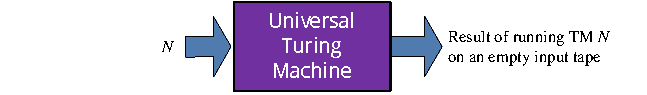
\includegraphics[width=4.8in]{figures/universal-machine.pdf}
\caption{Universal Turing Machine.}\label{fig:universalmachine}
\end{center}
\end{figure}

Since a Universal Turing Machine can simulate every Turing Machine, and a Turing Machine can perform any computation according to our intuitive notion of computation, this means a Universal Turing Machine can perform all computations.  Using the universal machine and a diagonalization argument similar to the one above for the real numbers, Turing reached a similar contradiction for a problem analogous to the Halting Problem for Python programs but for Turing Machines instead.

If we can simulate a Universal Turing Machine in a programming language, that language is a \definition{universal programming language}.  There is some program that can be written in that language to perform every possible computation.  

To show that a programming language is universal, it is sufficient to show that it can simulate any Turing Machine, since a Turing Machine can perform every possible computation.  To simulate a Universal Turing Machine, we need some way to keep track of the state of the tape (for example, the list datatypes in Scheme or Python would be adequate), a way to keep track of the internal machine state (a number can do this), and a way to execute the transition rules (we could define a procedure that does this using an if expression to make decisions about which transition rule to follow for each step), and a way to keep going (we can do this in Scheme with recursive applications).  Thus, Scheme is a universal programming language: one can write a Scheme program to simulate a Universal Turing Machine, and thus, perform any mechanical computation.

\section{Proving Non-Computability}\label{sec:noncomputability}

We can show that a problem is computable by describing a procedure and proving that the procedure always terminates and always produces the correct answer.  It is enough to provide a convincing argument that such a procedure exists; finding the actual procedure is not necessary (but often helps to make the argument more convincing).  

To show that a problem is not computable, we need to show that \emph{no} algorithm exists that solves the problem.  Since there are an infinite number of possible procedures, we cannot just list all possible procedures and show why each one does not solve the problem.  Instead, we need to construct an argument showing that if there were such an algorithm it would lead to a contradiction.  

The core of our argument is based on knowing the Halting Problem is noncomputable.  If a solution to some new problem $P$ could be used to solve the Halting Problem, then we know that $P$ is also noncomputable.  That is, no algorithm exists that can solve $P$ since if such an algorithm exists it could be used to also solve the Halting Problem which we already know is impossible.  

\shortsection{Reduction Proofs}  The proof technique where we show that a solution for some problem $P$ can be used to solve a different problem $Q$ is known as a \definition{reduction}.  

A problem $Q$ is \definition{reducible} to a problem $P$ if a solution to $P$ could be used to solve $Q$.  This means that problem $Q$ is no harder than problem $P$, since a solution to problem $Q$ leads to a solution to problem $P$.  

\begin{examplenobar}{Prints-Three Problem}  Consider the problem of determining if an application of a procedure would ever print \pycode|3|:

\problem{Prints-Three}{A string representing a Python program.}{If evaluating the input program would print \snumber{3}, output \True; otherwise, output \False.}

We show the Prints-Three Problem is noncomputable by showing that it is as hard as the Halting Problem, which we already know is noncomputable.  

Suppose we had an algorithm \pycode|printsThree| that solves the Prints-Three Problem.  Then, we could define \pycode|halts| as:
\begin{pythoncode}
def halts(p): 
   return printsThree(p +  '; print(3)')
\end{pythoncode}
The \pycode|printsThree| application would evaluate to \True\ if evaluating the Python program specified by \pycode|p| would halt since that means the \pycode|print(3)| statement appended to \pycode|p| would be evaluated.  On the other hand, if evaluating \pycode|p| would not halt, the added print statement never evaluated.  As long as the program specified by \pycode|p| would never print \pycode|3|, the application of \pycode|printsThree| should evaluate to \False.  Hence, if a \pycode|printsThree| algorithm exists, we would use it to implement an algorithm that solves the Halting Problem.

The one wrinkle is that the specified input program might print \pycode|3| itself.  We can avoid this problem by transforming the input program so it would never print \pycode|3| itself, without otherwise altering its behavior.  One way to do this would be to replace all occurrences of \pycode|print| (or any other built-in procedure that prints) in the string with a new procedure, \pycode|dontprint| that behaves like \pycode|print| but doesn't actually print out anything.  Suppose the \pycode|replacePrints| procedure is defined to do this.  Then, we could use \pycode|printsThree| to define \pycode|halts|:
\begin{pythoncode}
def halts(p): return printsThree(replacePrints(p) +  '; print(3)')
\end{pythoncode}

We know that the Halting Problem is noncomputable, so this means the Prints-Three Problem must also be noncomputable.
\end{examplenobar}

\begin{exploration}{Virus Detection}\vspace*{0.5ex}\par

\index{general}{virus}
The Halting Problem and Prints-Three Problem are noncomputable, but do seem to be obviously important problems.  It is useful to know if a procedure application will terminate in a reasonable amount of time, but the Halting Problem does not answer that question.  It concerns the question of whether the procedure application will terminate in any finite amount of time, no matter how long it is.  This example considers a problem for which it would be very useful to have a solution for it one existed.

A virus is a program that infects other programs.  A virus spreads by copying its own code into the code of other programs, so when those programs are executed the virus will execute.  In this manner, the virus spreads to infect more and more programs.  A typical virus also includes a malicious payload so when it executes in addition to infecting other programs it also performs some damaging (corrupting data files) or annoying (popping up messages) behavior.  The Is-Virus Problem is to determine if a procedure specification contains a virus:

\problem{Is-Virus}{A specification of a Python program.}{If the expression contains a virus (a code fragment that will infect other files) output \True.  Otherwise, output \False.}

We demonstrate the Is-Virus Problem is noncomputable using a similar strategy to the one we used for the Prints-Three Problem: we show how to define a \pycode|halts| algorithm given a hypothetical \pycode|isVirus| algorithm.  Since we know \pycode|halts| is noncomputable, this shows there is no \pycode|isVirus| algorithm.  

Assume \pycode|infectFiles| is a procedure that infects files, so the result of evaluating \pycode|isVirus('infectFiles()')| is \True.  We could define \pycode|halts| as:

\begin{pythoncode}
def halts(p): 
   return isVirus(p + '; infectFiles()')
\end{pythoncode}

This works as long as the program specified by \pycode|p| does not exhibit the file-infecting behavior.  If it does, \pycode|p| could infect a file and never terminate, and \pycode|halts| would produce the wrong output.  To solve this we need to do something like we did in the previous example to hide the printing behavior of the original program.  

A rough definition of file-infecting behavior would be to consider any write to an executable file to be an infection.  To avoid any file infections in the specific program, we replace all procedures that write to files with procedures that write to shadow copies of these files.  For example, we could do this by creating a new temporary directory and prepend that path to all file names.  We call this (assumed) procedure, \pycode|sandBox|, since it transforms the original program specification into one that would execute in a protected sandbox.

\begin{pythoncode}
def halts(p): isVirus(sandBox(p) + '; infectFiles()')
\end{pythoncode}

Since we know there is no algorithm that solves the Halting Problem, this proves that there is no algorithm that solves the Is-Virus problem.

Virus scanners such as Symantec's Norton AntiVirus attempt to solve the Is-Virus Problem, but its non-computability means they are doomed to always fail.  Virus scanners detect known viruses by scanning files for strings that match signatures in a database of known viruses.  As long as the signature database is frequently updated they may be able to detect currently spreading viruses, but this approach cannot detect a new virus that will not match the signature of a previously known virus.  

Sophisticated virus scanners employ more advanced techniques to attempt to detect complex viruses such as metamorphic viruses that alter their own code as they propagate to avoid detection.  But, because the general Is-Virus Problem is noncomputable, we know that it is impossible to create a program that always terminates and that always correctly determines if an input procedure specification is a virus.

\par
\end{exploration}

\beforeex
\begin{exercise}
Is the Launches-Missiles Problem described below computable?  Provide a convincing argument supporting your answer.

\problem{Launches-Missiles}{A specification of a procedure.}{If an application of the procedure would lead to the missiles being launched, outputs \True.  Otherwise, outputs \False.}

You may assume that the only thing that causes the missiles to be launched is an application of the \pycode|launchMissiles| procedure.
\solution{\LATER{}}
\end{exercise}
\afterex

\marginquote{I am rather puzzled why you draw this distinction between proof finders and proof checkers.  It seems to me rather unimportant as one can always get a proof finder from a proof checker, and the converse is almost true: the converse false if for instance one allows the proof finder to go through a proof in the ordinary way, and then, rejecting the steps, to write down the final formula as a 'proof' of itself.  One can easily think up suitable restrictions on the idea of proof which will make this converse true and which agree well with our ideas of what a proof should be like.  I am afraid this may be more confusing to you than enlightening.\cut{  If so I will try again.}}{Alan Turing, letter to Max Newman, 1940}

\beforeex
\begin{exercise}
Is the Same-Result Problem described below computable?  Provide a convincing argument supporting your answer.

\problem{Same-Result}{Specifications of two procedures, $P$ and $Q$.}{If an application of $P$ terminates and produces the same value as applying $Q$, outputs \True.  If an application of $P$ does not terminate, and an application of $Q$ also does not terminate, outputs \True.  Otherwise, outputs \False.}
\solution{\LATER{}}
\end{exercise}
\afterex

\beforesplitex
\begin{exercise}
Is the Check-Proof Problem described below computable?   Provide a convincing argument supporting your answer.

\problem{Check-Proof}{A specification of an axiomatic system, a statement (the theorem), and a proof (a sequence of steps, each identifying the axiom that is applied).}
{Outputs \True\ if the proof is a valid proof of the theorem in the system, or \False\ if it is not a valid proof.}
\solution{\LATER{}}
\end{exercise}
\aftersplitex

\beforesplitex
\begin{exercise}
Is the Find-Finite-Proof Problem described below computable?   Provide a convincing argument supporting your answer.

\problem{Find-Finite-Proof}{A specification of an axiomatic system, a statement (the theorem), and a maximum number of steps (max-steps).}
{If there is a proof in the axiomatic system of the theorem that uses max-steps or fewer steps, outputs \True.  Otherwise, outputs \False.}
\solution{\LATER{}}
\end{exercise}
\aftersplitex

\beforeex
\begin{exercise}\goldstar
Is the Find-Proof Problem described below computable?   Provide a convincing argument why it is or why it is not computable.

\problem{Find-Proof}{A specification of an axiomatic system, and a statement (the theorem).}
{If there is a proof in the axiomatic system of the theorem, outputs \True.  Otherwise, outputs \False.}
\solution{\LATER{}}
\end{exercise}
\afterex


\begin{exploration}{Busy Beavers}\vspace*{0.5ex}\par

\index{general}{busy beaver problem}Consider the Busy-Beaver Problem (devised by Tibor Rad\'{o}\index{people}{Rad\'{o}, Tibor} in 1962):

\problem{Busy-Beaver}{A positive integer, $n$.}{A number representing that maximum number of steps a Turing Machine with $n$ states and a two-symbol tape alphabet can run starting on an empty tape before halting.}

We use $0$ and $1$ for the two tape symbols, where the blank squares on the tape are interpreted as $0$s (alternately, we could use \emph{blank} and \emph{X} as the symbols, but it is more natural to describe machines where symbols are $0$ and $1$, so we can think of the initially blank tape as containing all $0$s).

For example, if the Busy Beaver input $n$ is $1$, the output should be $1$.  The best we can do with only one state is to halt on the first step.  If the transition rule for a $0$ input moves left, then it will reach another $0$ square and continue forever without halting; similarly it if moves right.   

For $n = 2$, there are more options to consider.  The machine in Figure~\ref{fig:bb} runs for 6 steps before halting, and there is no two-state machine that runs for more steps.  One way to support this claim would be to try simulating all possible two-state Turing Machines.  

\begin{figure}[!bh]
\begin{center}
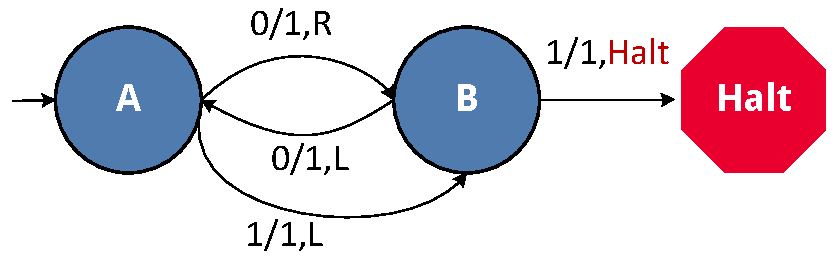
\includegraphics[width=3.5in]{figures/tm-bb.pdf}
\caption{Two-state Busy Beaver Machine.}\label{fig:bb}
\end{center}
\end{figure}

Busy Beaver numbers increase extremely quickly.  The maximum number of steps for a three-state machine is 21, and for a four-state machine is 107.  The value for a five-state machine is not yet known, but the best machine found to date runs for 47,176,870 steps!  For six states, the best known result, discovered in 2007 by Terry Ligocki and Shawn Ligocki, is over 2879 decimal digits long.

We can prove the Busy Beaver Problem is noncomputable by reducing the Halting Problem to it.  Suppose we had an algorithm, \pycode|bb(n)|, that takes the number of states as input and outputs the corresponding Busy Beaver.  Then, we could solve the Halting Problem for a Turing Machine:

\problem{TM Halting Problem}{A string representing a Turing Machine.}{If executing the input Turing Machine starting with a blank tape would ever finish, output \True.  Otherwise, output \False.}

The TM Halting Problem is different from the Halting Problem as we defined it earlier, so first we need to show that the TM Halting Problem is noncomputable by showing it could be used to solve the Python Halting Problem.  Because Python is universal programming language, it is possible to transform any Turing Machine into a Python program.  Once way to do this would be to write a Universal Turing Machine simulator in Python, and then create a Python program that first creates a tape containing the input Turing Machine description, and then calls the Universal Turing Machine simulator on that input.  This shows that the TM Halting Problem is noncomputable.

Next, we show that an algorithm that solves the Busy Beaver Problem could be used to solve the TM Halting Problem.  Here's how (in Pythonish pseudocode):
\begin{pythoncode}
def haltsTM(m):
   states = numberOfStates(m)
   maxSteps = bb(states)
   state = 0
   tape = []
   for step in range(0, maxSteps):
      state, tape = simulateOneStep(m, state, tape)
      if halted(state): return True
   return False      
\end{pythoncode}
The \pycode|simulateOneStep| procedure takes as inputs a Turing Machine description, its current state and tape, and simulates the next step on the machine.  So, \pycode|haltsTM| simulates up to $bb(n)$ steps of the input machine $m$ where $n$ is the number of states in $m$.  Since $bb(n)$ is the maximum number of steps a Turing Machine with $n$ states can execute before halting, we know if $m$ has not halted in the simulate before \pycode|maxSteps| is reached that the machine $m$ will never halt, and can correctly return \False.  This means there is no algorithm that can solve the Busy Beaver Problem.

\beforeex
\begin{exercise}
Confirm that the machine showing in Figure~\ref{fig:bb} runs for 6 steps before halting.
\solution{\LATER{}}
\end{exercise}
\afterex


\beforeex
\begin{exercise}
Prove the Beaver Bound problem described below is also noncomputable:

\problem{Beaver-Bound}{A positive integer, $n$.}{A number that is greater than the maximum number of steps a Turing Machine with $n$ states and a two-symbol tape alphabet can run starting on an empty tape before halting.}

A valid solution to the Beaver-Bound problem can produce any result for $n$ as long as it is greater than the Busy Beaver value for $n$.
\solution{\LATER{}}
\end{exercise}
\afterex

\beforeex
\begin{exercise}
\triplegoldstar Find a 5-state Turing Machine that runs for more than 47,176,870 steps, or prove that no such machine exists.
\solution{\LATER{}}
\end{exercise}
\afterex


\end{exploration}


\section{Summary}

Although today's computers can do amazing things, many of which could not even have been imagined twenty years ago, there are problems that can never be solved by computing.  The Halting Problem is the most famous example: it is impossible to define a mechanical procedure that always terminates and correctly determines if the computation specified by its input would terminate.  Once we know the Halting Problem is noncomputable, we can show that other problems are also noncomputable by illustrating how a solution to the other problem could be used to solve the Halting Problem which we know to be impossible.  

Noncomputable problems frequently arise in practice.  For example, identifying viruses, analyzing program paths, and constructing proofs, are all noncomputable problems.  

Just because a problem is noncomputable does not mean we cannot produce useful programs that address the problem.  These programs provide approximate solutions, which are often useful in practice.  They produce the correct results on many inputs, but on some inputs must either fail to produce any result or produce an incorrect result.  
%Approximate solutions are often useful in practice, however, even if it is impossible to solve the problem.  

\end{schemeregion}